\documentclass{templateNote}
\usepackage{soul}

\begin{document}

\imagenlogoU{img/LogoElNube.png}
\linklogoU{https://github.com/MarceloPazPezo}
\imagenlogoD{img/LogoNGM.png}
\linklogoD{https://github.com/NicoGomezM}
\linkQRDoc{https://github.com/MarceloPazPezo/MyRepo/blob/main/Icinf/Semestre\%207/Sistemas\%20de\%20Informaci\%C3\%B3n/Test\%203/Test-3.pdf}
\titulo{Test 3}
\asignatura{Sistemas de Informaci\'on}
\autor{
Marcelo Paz\\
Nicol\'as G\'omez
}
\vDoc{1.1.0}

% Metadatos del PDF
\title{[\asignatura]-\titulo}
\author{
    \autor
}
\portada
\margenes % Crear márgenes

\section{Diagramas de flujo de datos (\textbf{DFD})} 
\noindent Los diagramas de flujo de datos son una herramienta que nos permite modelar procesos y mostrar como se mueve la información. Dentro de los DFD existen 3 niveles:
\begin{itemize}
    \item Diagrama de contexto: Muestra el sistema como una caja negra y las interacciones que tiene con el entorno (No muestra archivos).
    \begin{figure}[H]
        \centering
        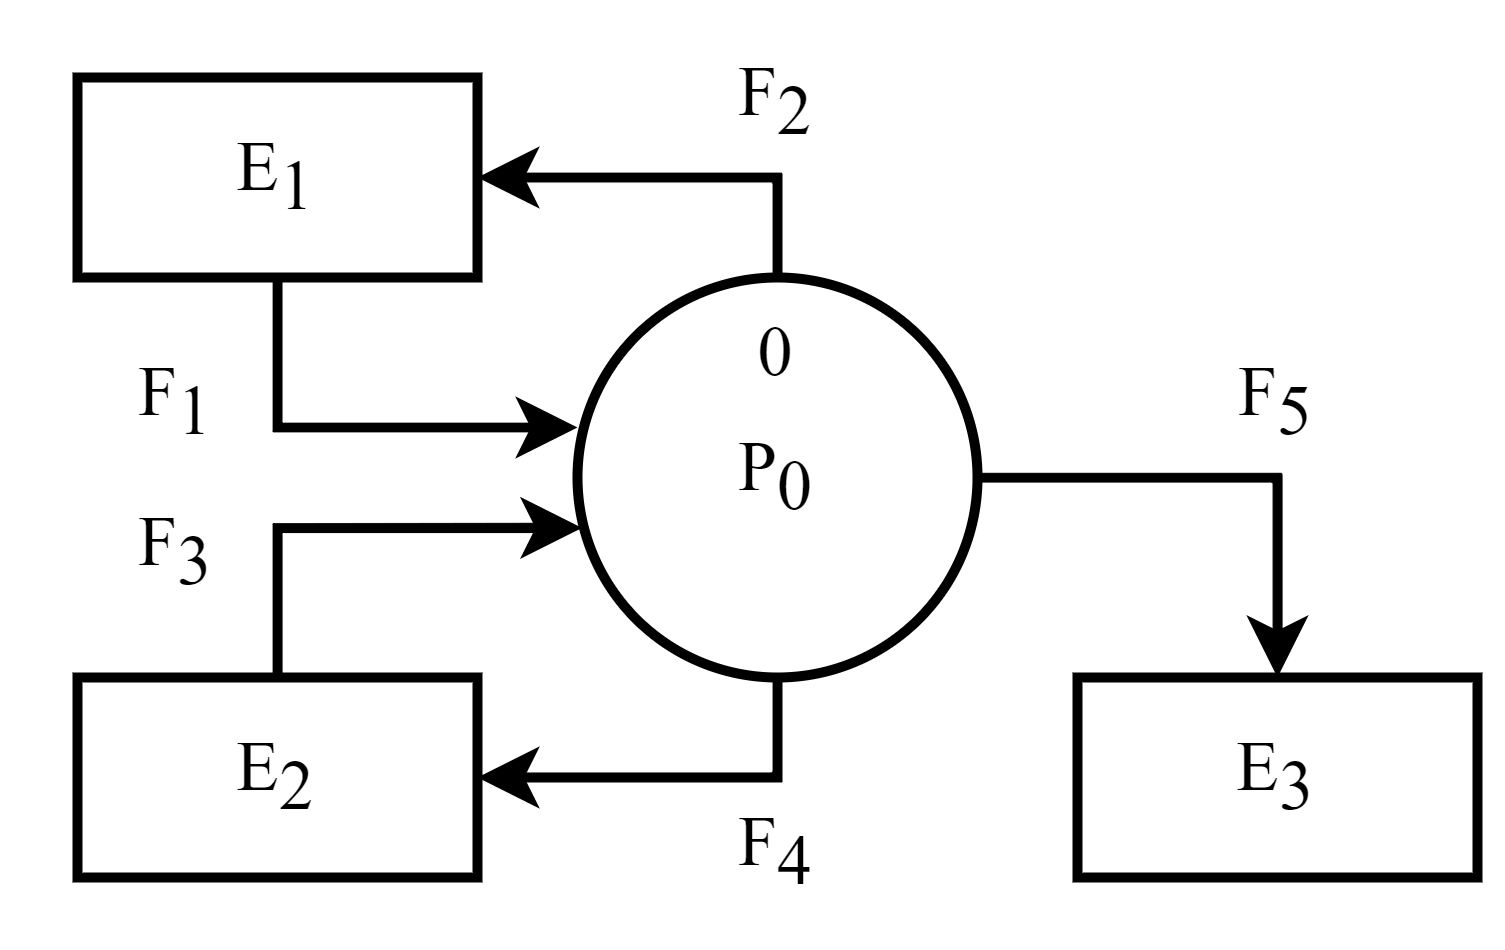
\includegraphics[width=0.4\textwidth]{diagram/DFD-Contexto.png}
    \end{figure}

    \item Diagrama de nivel superior: Muestra a detalle los procesos y elementos pertenecientes al diagrama de contexto, incluyendo archivos y bases de datos (Muestra archivos).
    \begin{figure}[H]
        \centering
        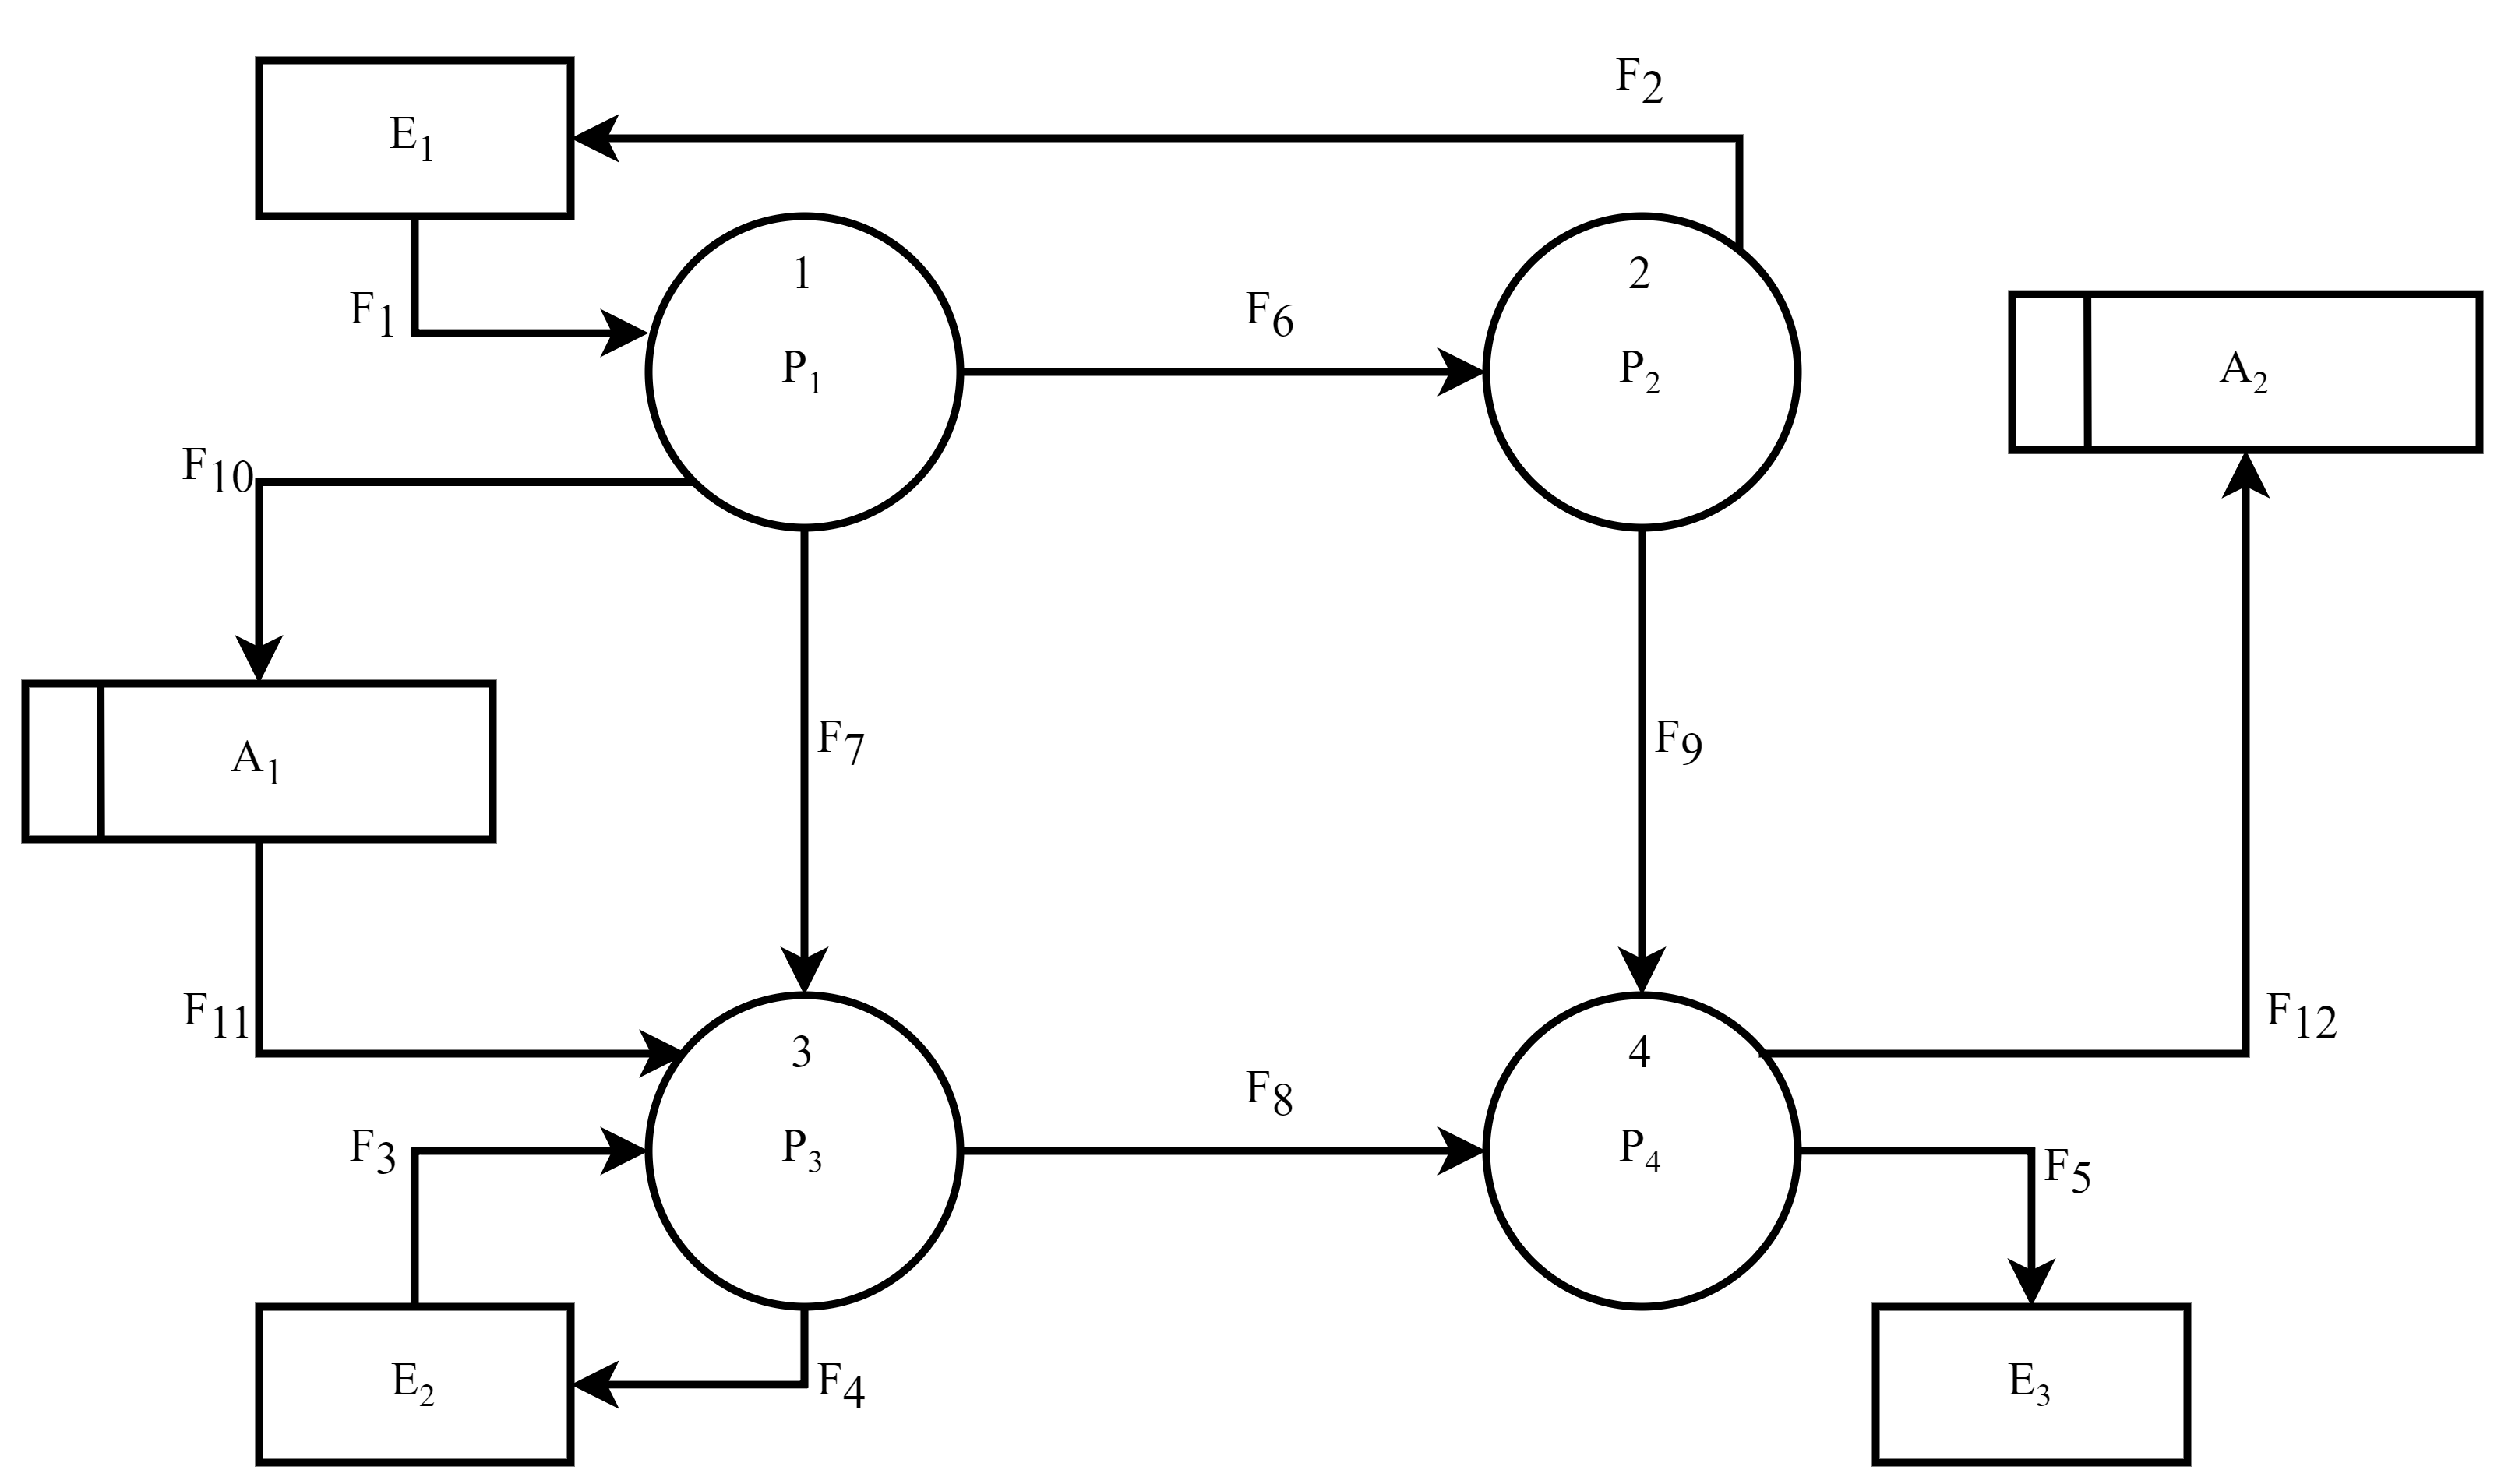
\includegraphics[width=0.8\textwidth]{diagram/DFD-Superior.png}
    \end{figure}
    
    \item Diagrama de detalle o expansion: Muestra a detalle los procesos y elementos pertenecientes al diagrama de nivel superior (Conserva archivos y entidades; Procesos superiores se representan de otra forma).
    \begin{figure}[H]
        \centering
        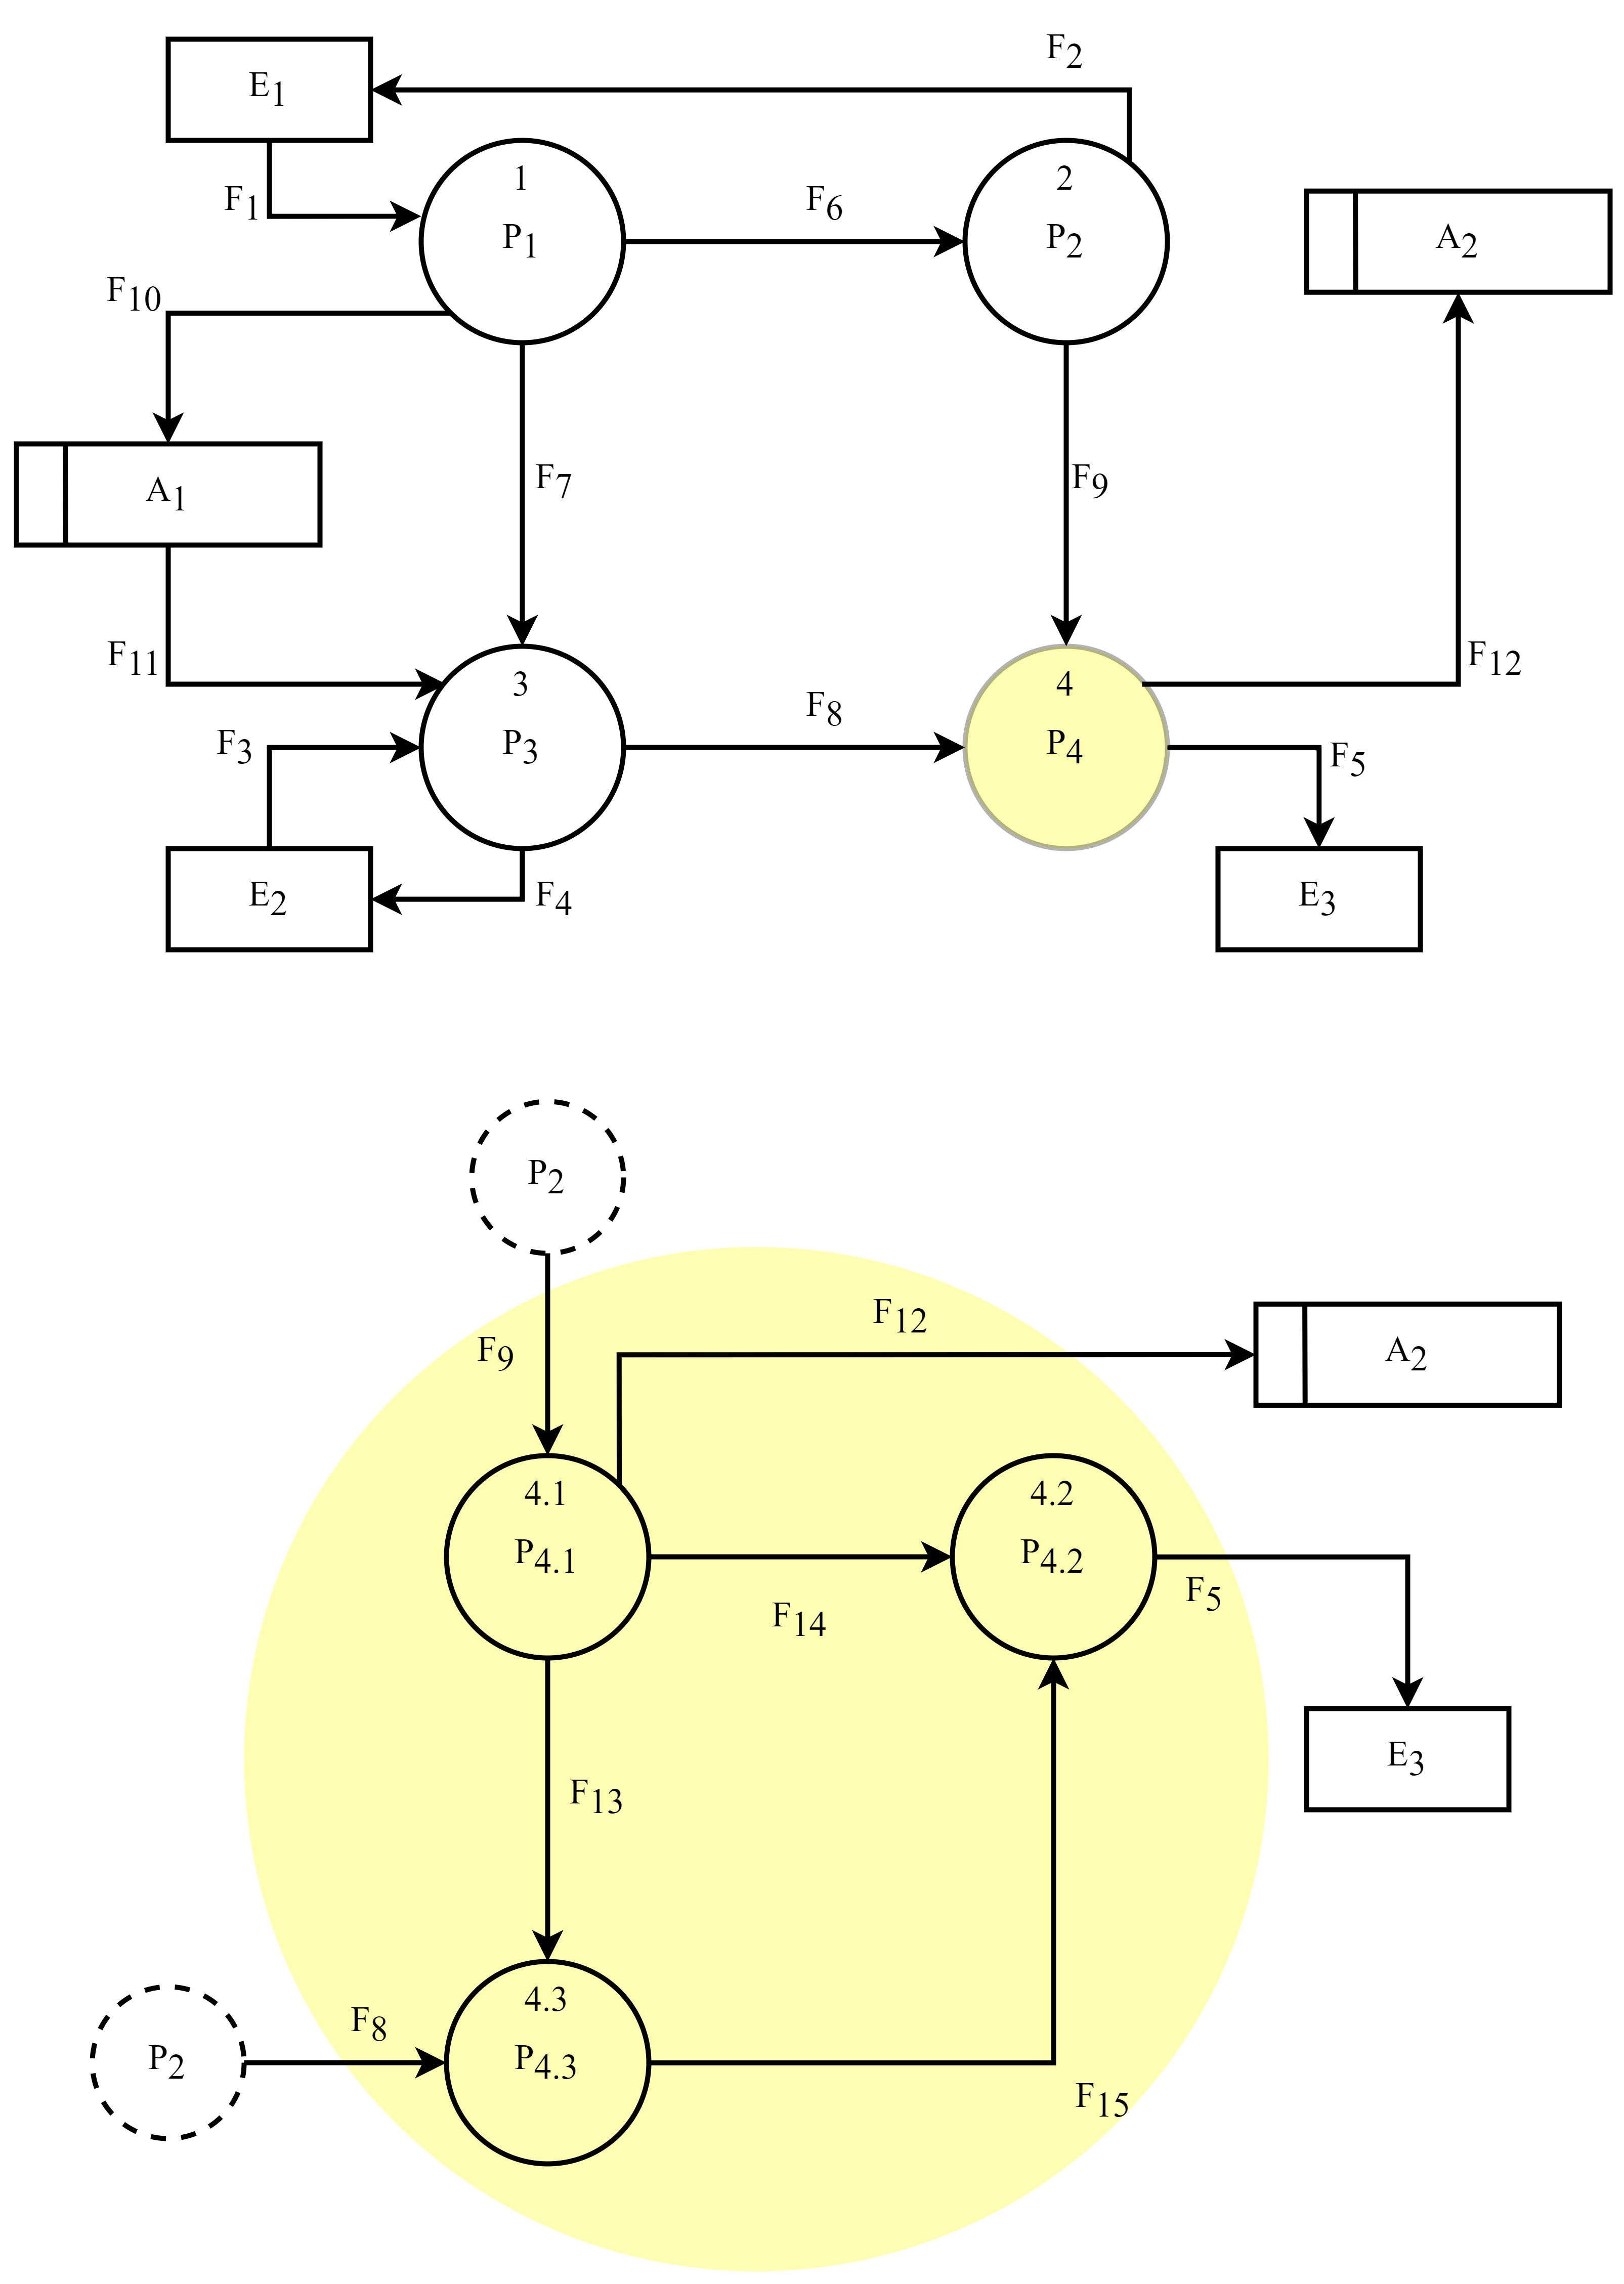
\includegraphics[width=0.9\textwidth]{diagram/DFD-Detallado.png}
    \end{figure}
\end{itemize}

\newpage
Las figuras que utilizaremos para la construcción de nuestros DFD son:
\begin{figure}[H]
    \centering
    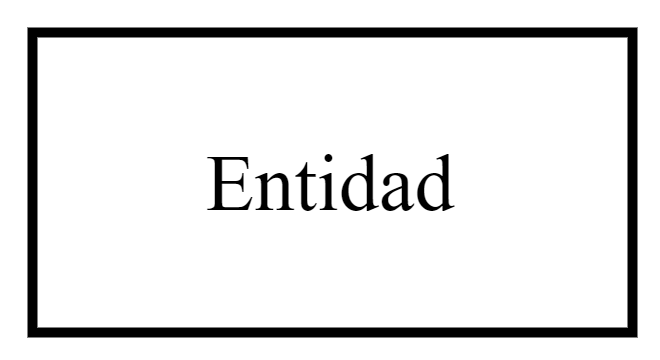
\includegraphics[width=0.3\textwidth]{diagram/Entidad.png}\hspace{1.5cm}
    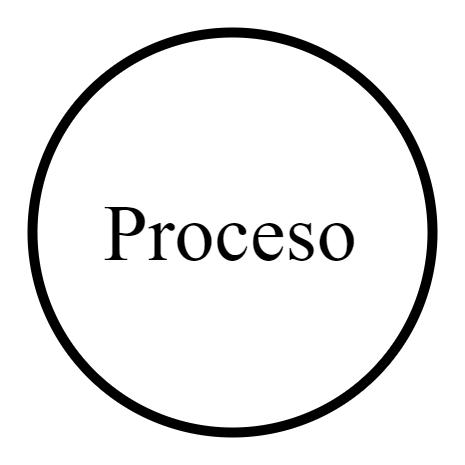
\includegraphics[width=0.2\textwidth]{diagram/Proceso.png}\hspace{1.5cm}
    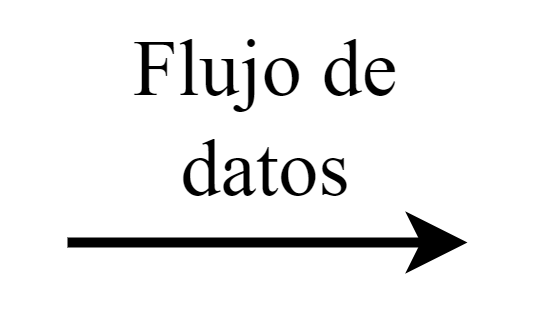
\includegraphics[width=0.27\textwidth]{diagram/Flujo.png}\hspace{1.5cm}
\end{figure}

\begin{figure}[H]
    \centering
    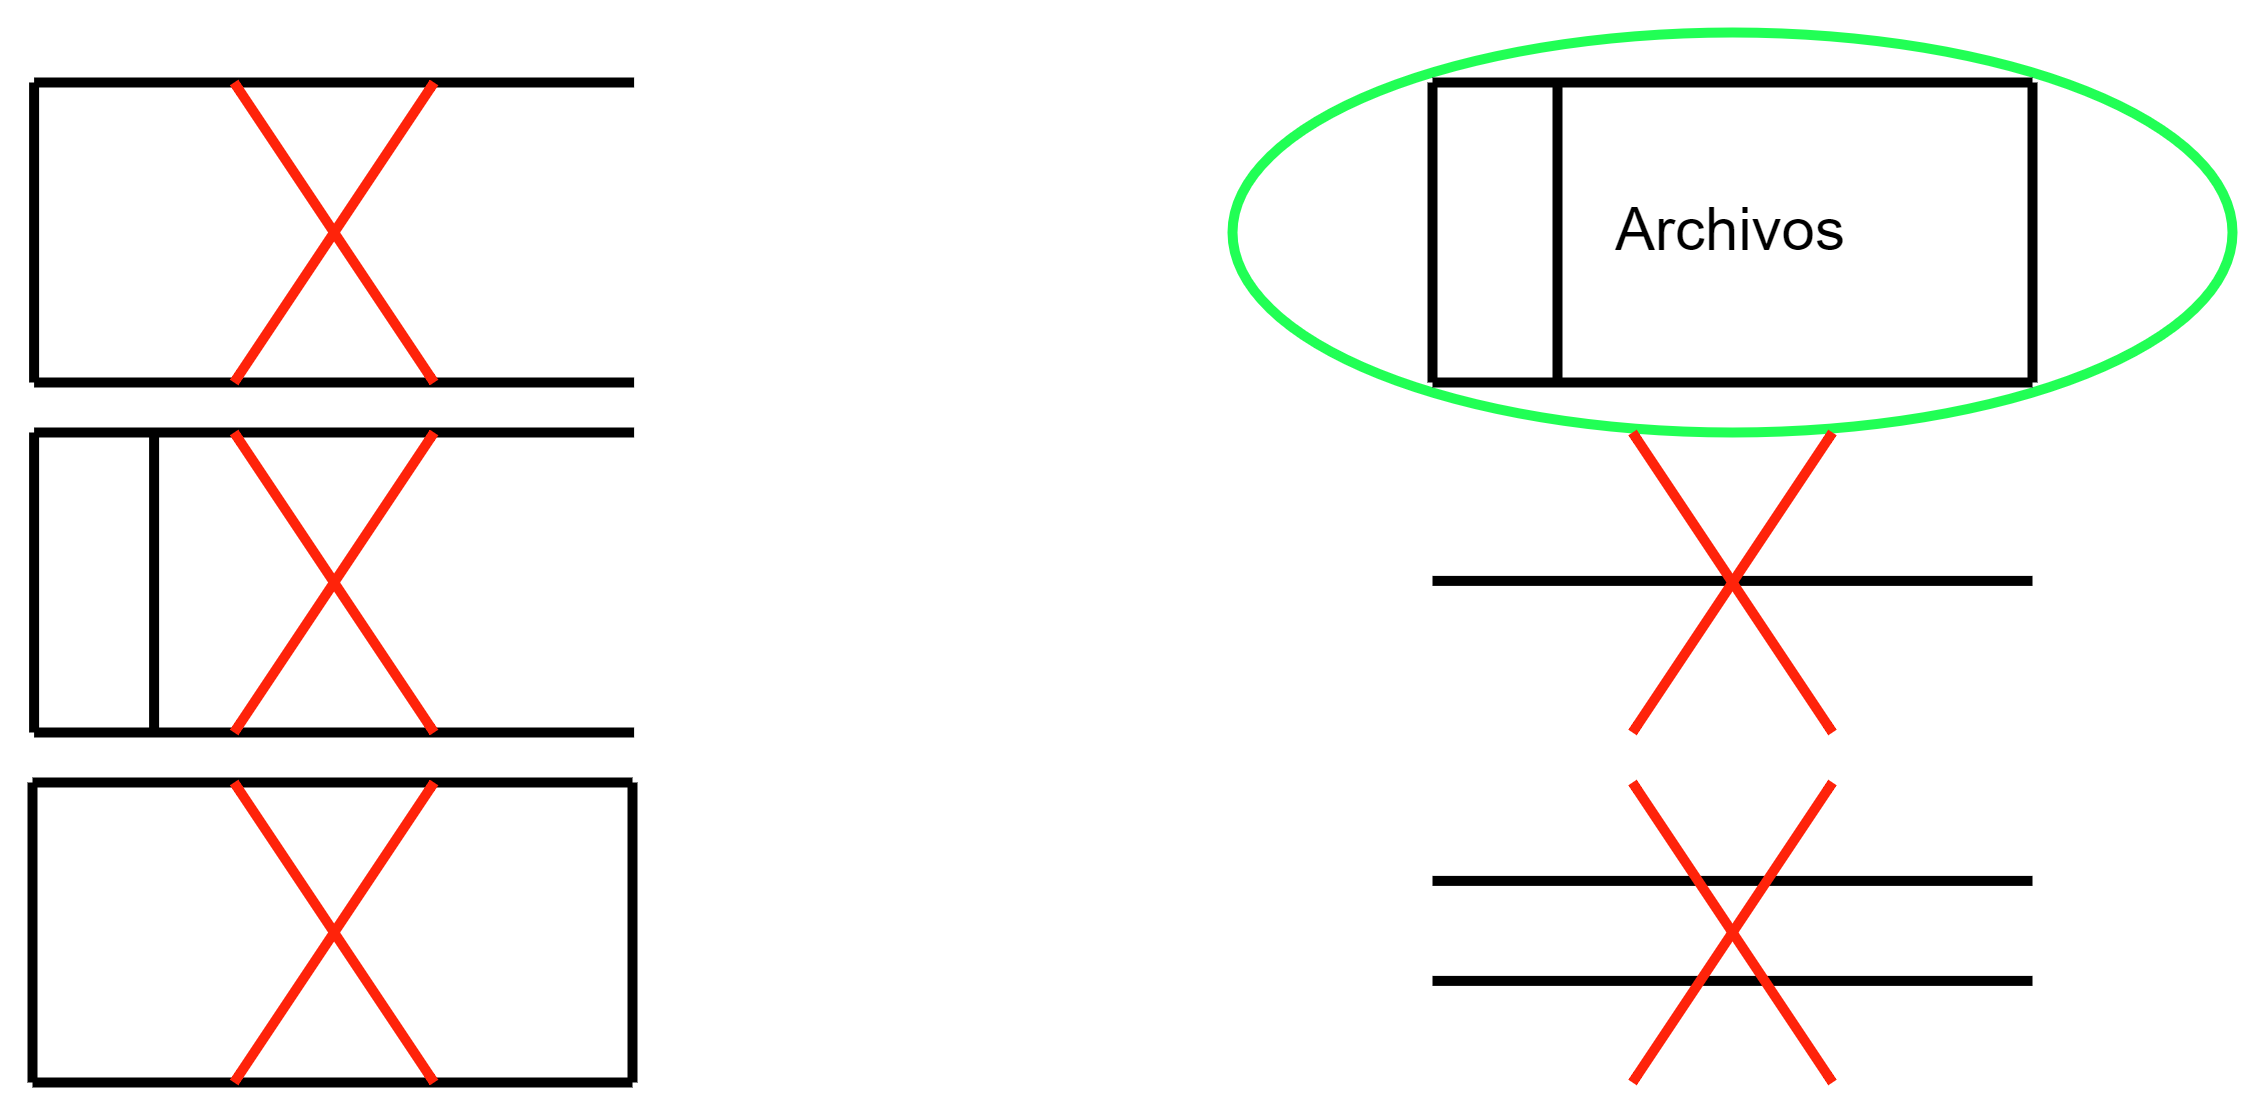
\includegraphics[width=0.6\textwidth]{diagram/Archivo.png}
\end{figure}

\subsection{Características generales de los elementos de un DFD}
\noindent\textbf{Entidades:} Son los elementos que generan o consumen información.
\begin{itemize}
    \item No existen relaciones (flujos) entre entidades.
    
    \item Se pueden repetir entidades colocando una linea diagonal en la esquina superior derecha por cada copia.
\end{itemize}
\textbf{Procesos:} Son las actividades que se realizan sobre la información.
\begin{itemize}
    \item Nombres de los procesos terminan en verbo o en -ción.
\end{itemize}
\textbf{Flujos:} Son las flechas que indican el movimiento de la información.
\begin{itemize}
    \item Nombre de los flujos \textbf{NO} comienzan por verbo \\(Ej.: Devolución libro $\rightarrow$ Libro devuelto).
    
    \item Nombres de flujos de archivos en formato: ``información.requerida-nombre.archivo''.
    
    \item Nombre de flujos no se pueden repetir.
    
    \item Elementos son flujos de datos.
    
    \item Lineas de flujo no se cruzan.
    
    \item No son acciones.
    
    \item Evitar redundancias.
\end{itemize}
\textbf{Archivos:} Son los almacenes de información.
\begin{itemize}
    \item Archivos se relacionan con procesos y no con entidades
    
    \item Archivos no se relacionan entre si.
\end{itemize}
\subsubsection{Identificación de entidades}
\begin{enumerate}
    \item Todo aquel que aporte algún dato al proceso y que no forme parte del proceso es entidad.
    
    \item Todo aquel que reciba información del proceso y que no forme parte del proceso es entidad.
    
    \item Todo aquel que lleve a cabo el proceso, que este a cargo del proceso y/o forma parte del proceso, no es entidad.
\end{enumerate}

\newpage
\subsection{Ejercicio 1}
Usted a aprobado todo el semestre y para celebrarlo a decidido invitar a algunos de sus compañeros a un asado en su casa, para ello llevará a cabo la planificación de un asado, por lo que para mayor claridad llevara a cabo el modelo de un DFD de contexto y nivel superior.\\
\textbf{Requerimientos:}
\begin{itemize}
    \item El asado se llevará a cabo en la casa, por lo tanto el arrendar un lugar no es necesario.
    
    \item Se invitarán a algunos de los compañeros, por lo que realizará una lista de invitados (Se filtran los compañeros).
    
    \item Se comprará carne, carbón, e insumos para el asado, por lo que realizará una lista de compras (Se necesitan datos sobre un asado).
\end{itemize}

\subsubsection{Diagrama de contexto}
\begin{figure}[H]
    \centering
    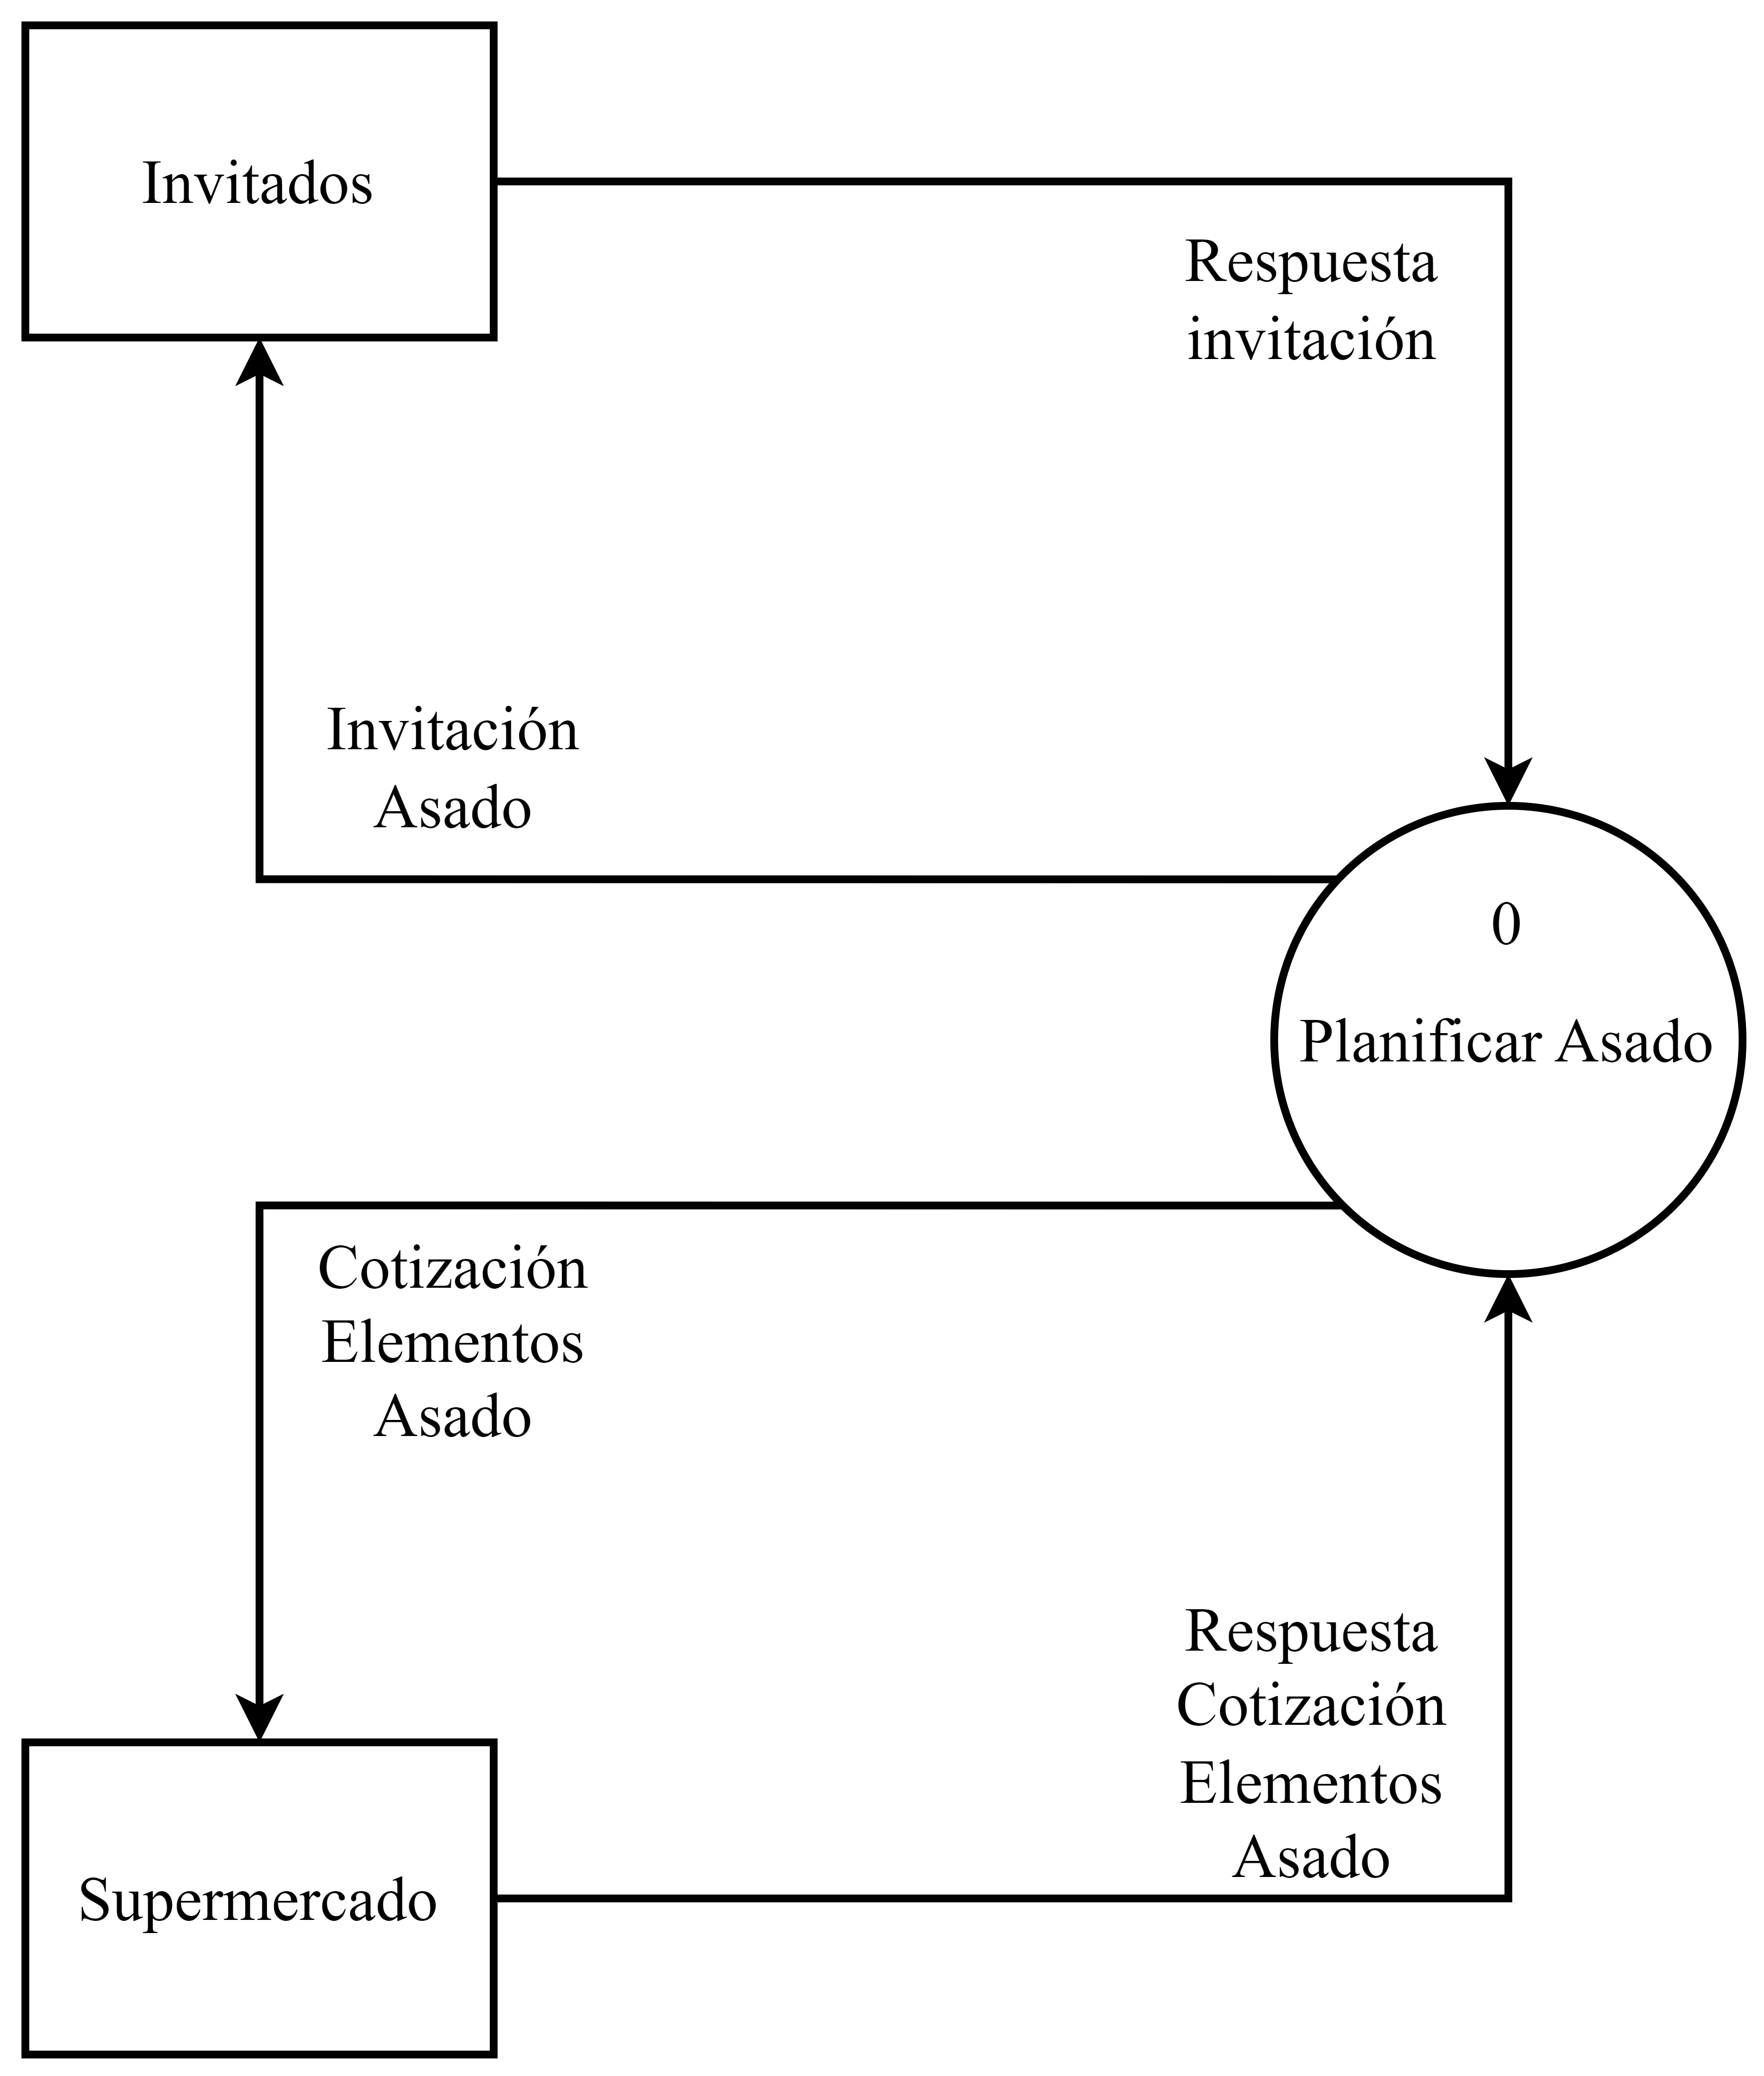
\includegraphics[width=0.6\textwidth]{diagram/DFD1-Contexto.png}
\end{figure}

\newpage
\subsubsection{Diagrama de nivel superior}
\begin{figure}[H]
    \centering
    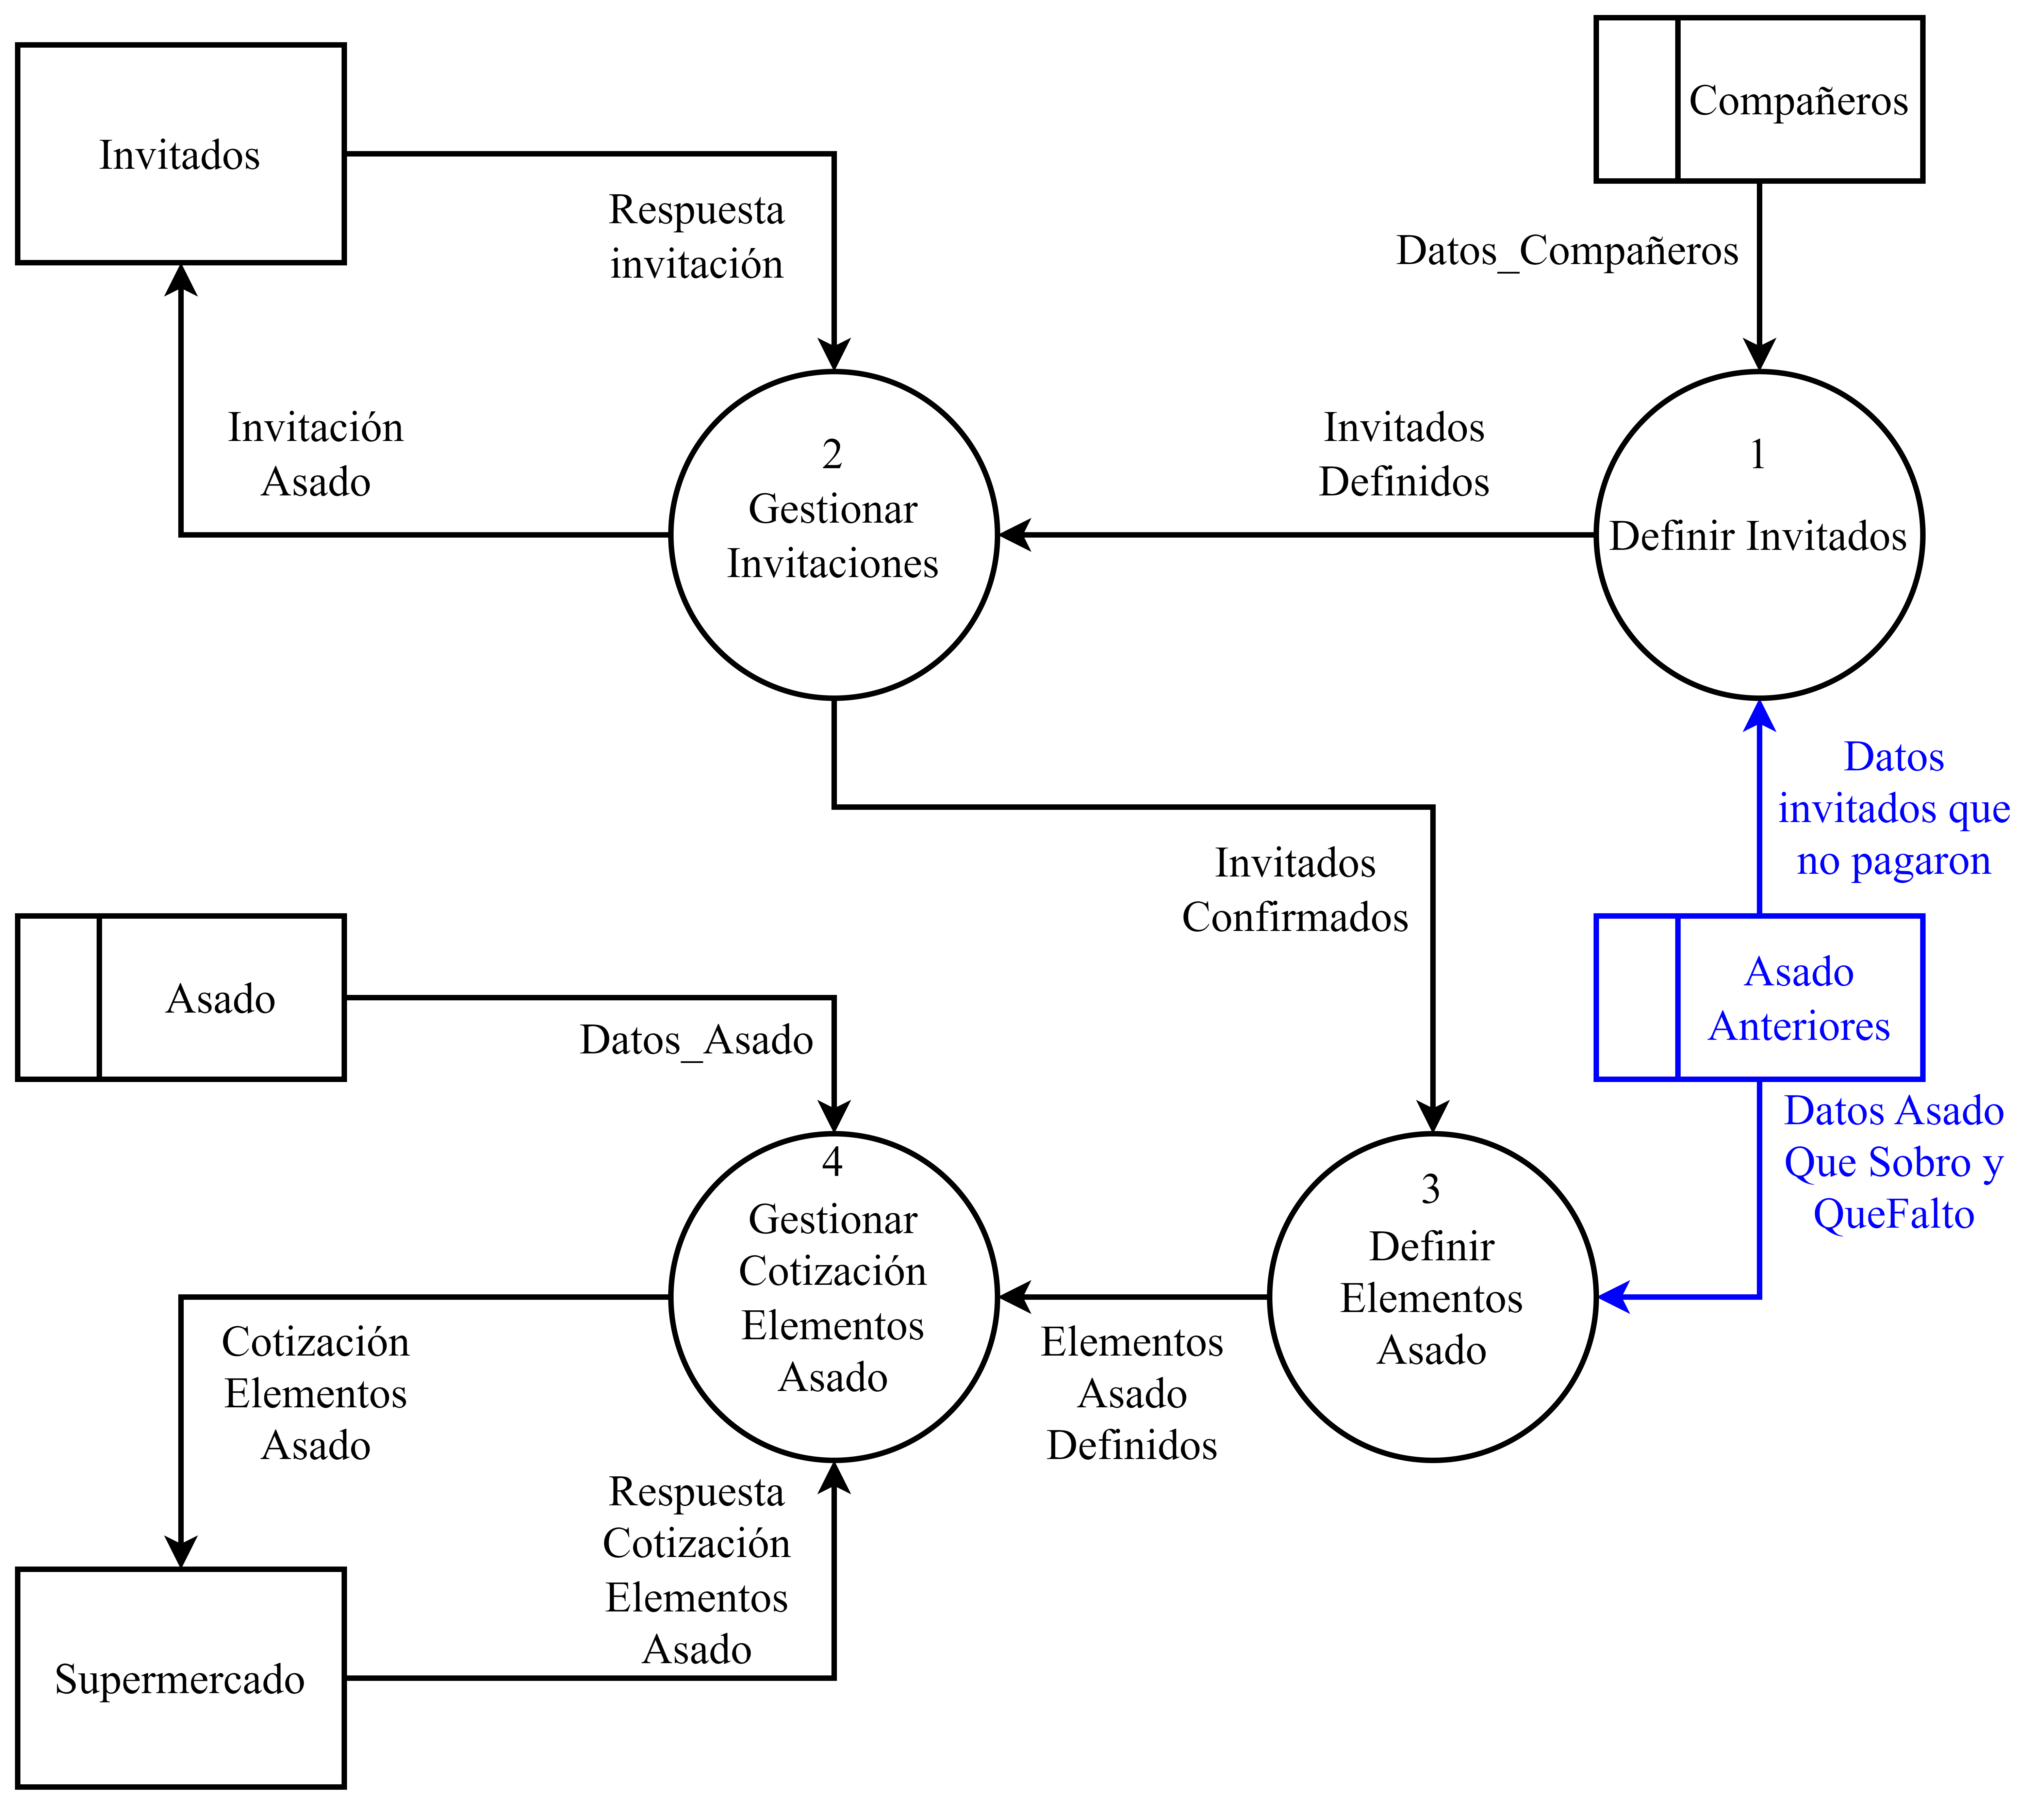
\includegraphics[width=0.9\textwidth]{diagram/DFD1-Superior.png}
\end{figure}
*OBS: Lo que se muestra en azul fue agregado por el profesor en el momento.

\newpage
\subsection{Ejercicio 2}
Hacer un DFD del punto de vista de una biblioteca universitaria, donde se muestre el proceso de préstamo de libros a sus usuarios.
\subsubsection{Diagrama de contexto}
\begin{figure}[H]
    \centering
    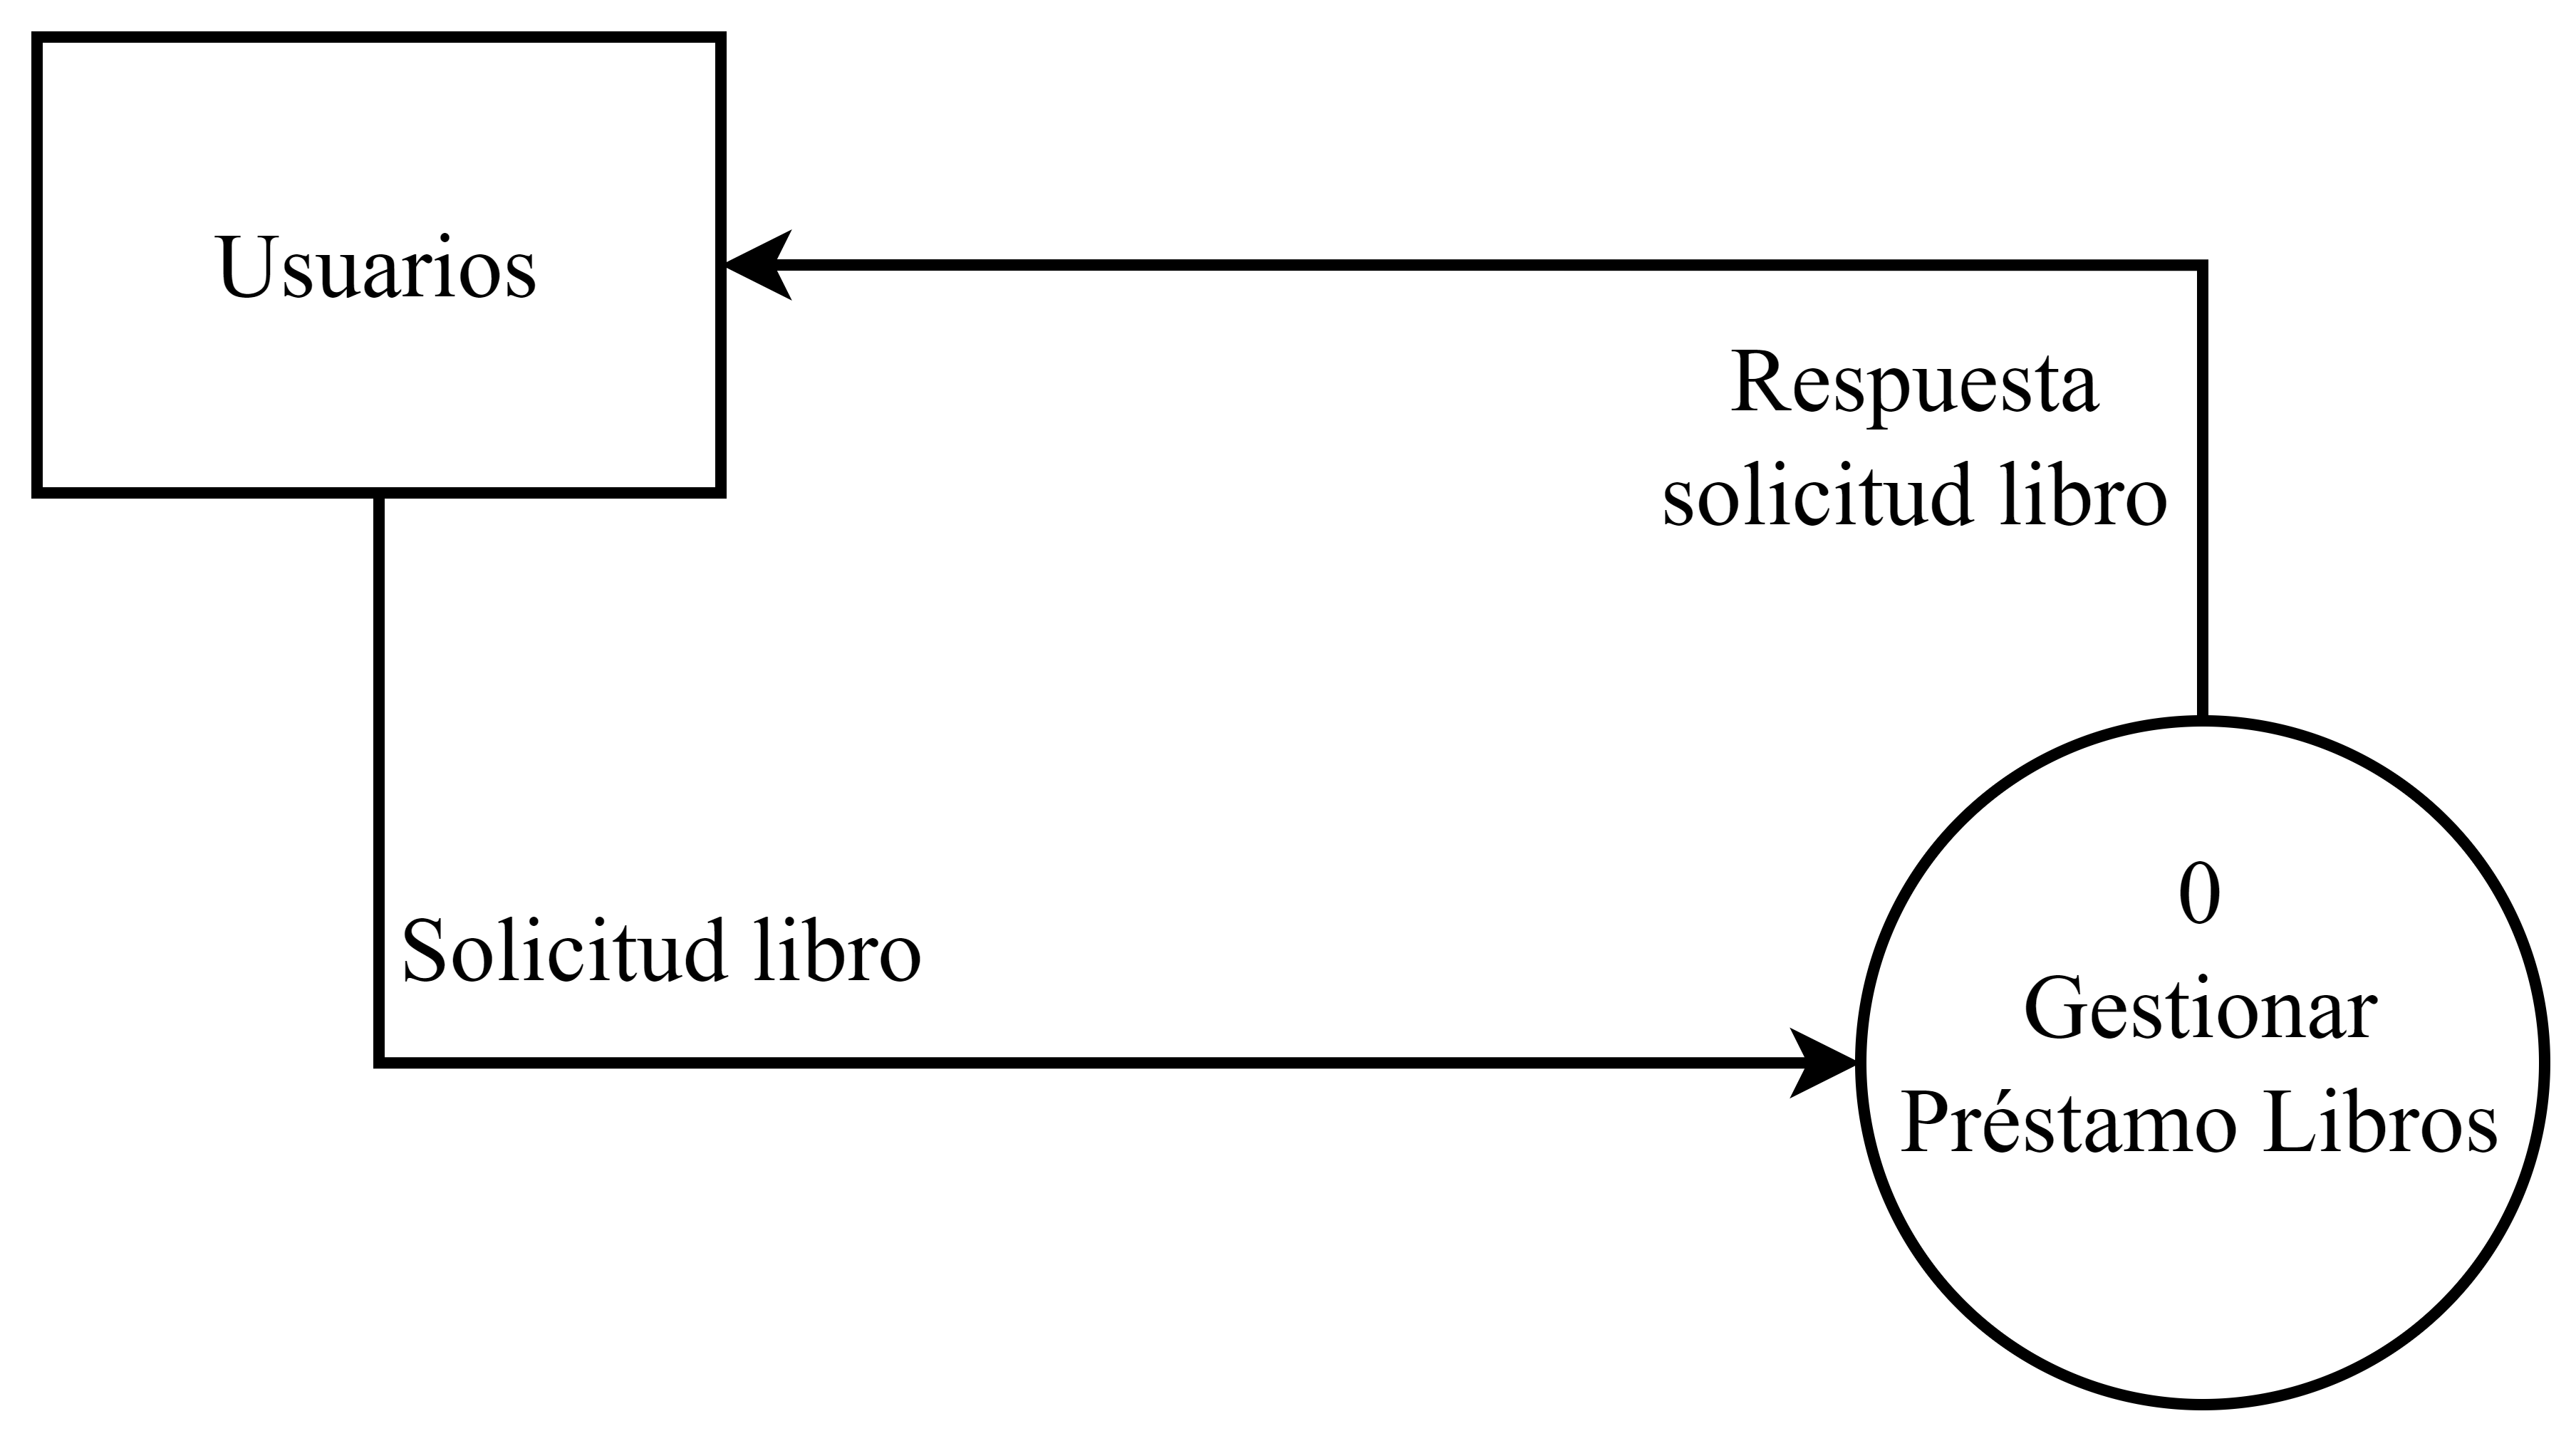
\includegraphics[width=0.6\textwidth]{diagram/DFD2-Contexto.png}
\end{figure}

\subsubsection{Diagrama de nivel superior}
\begin{figure}[H]
    \centering
    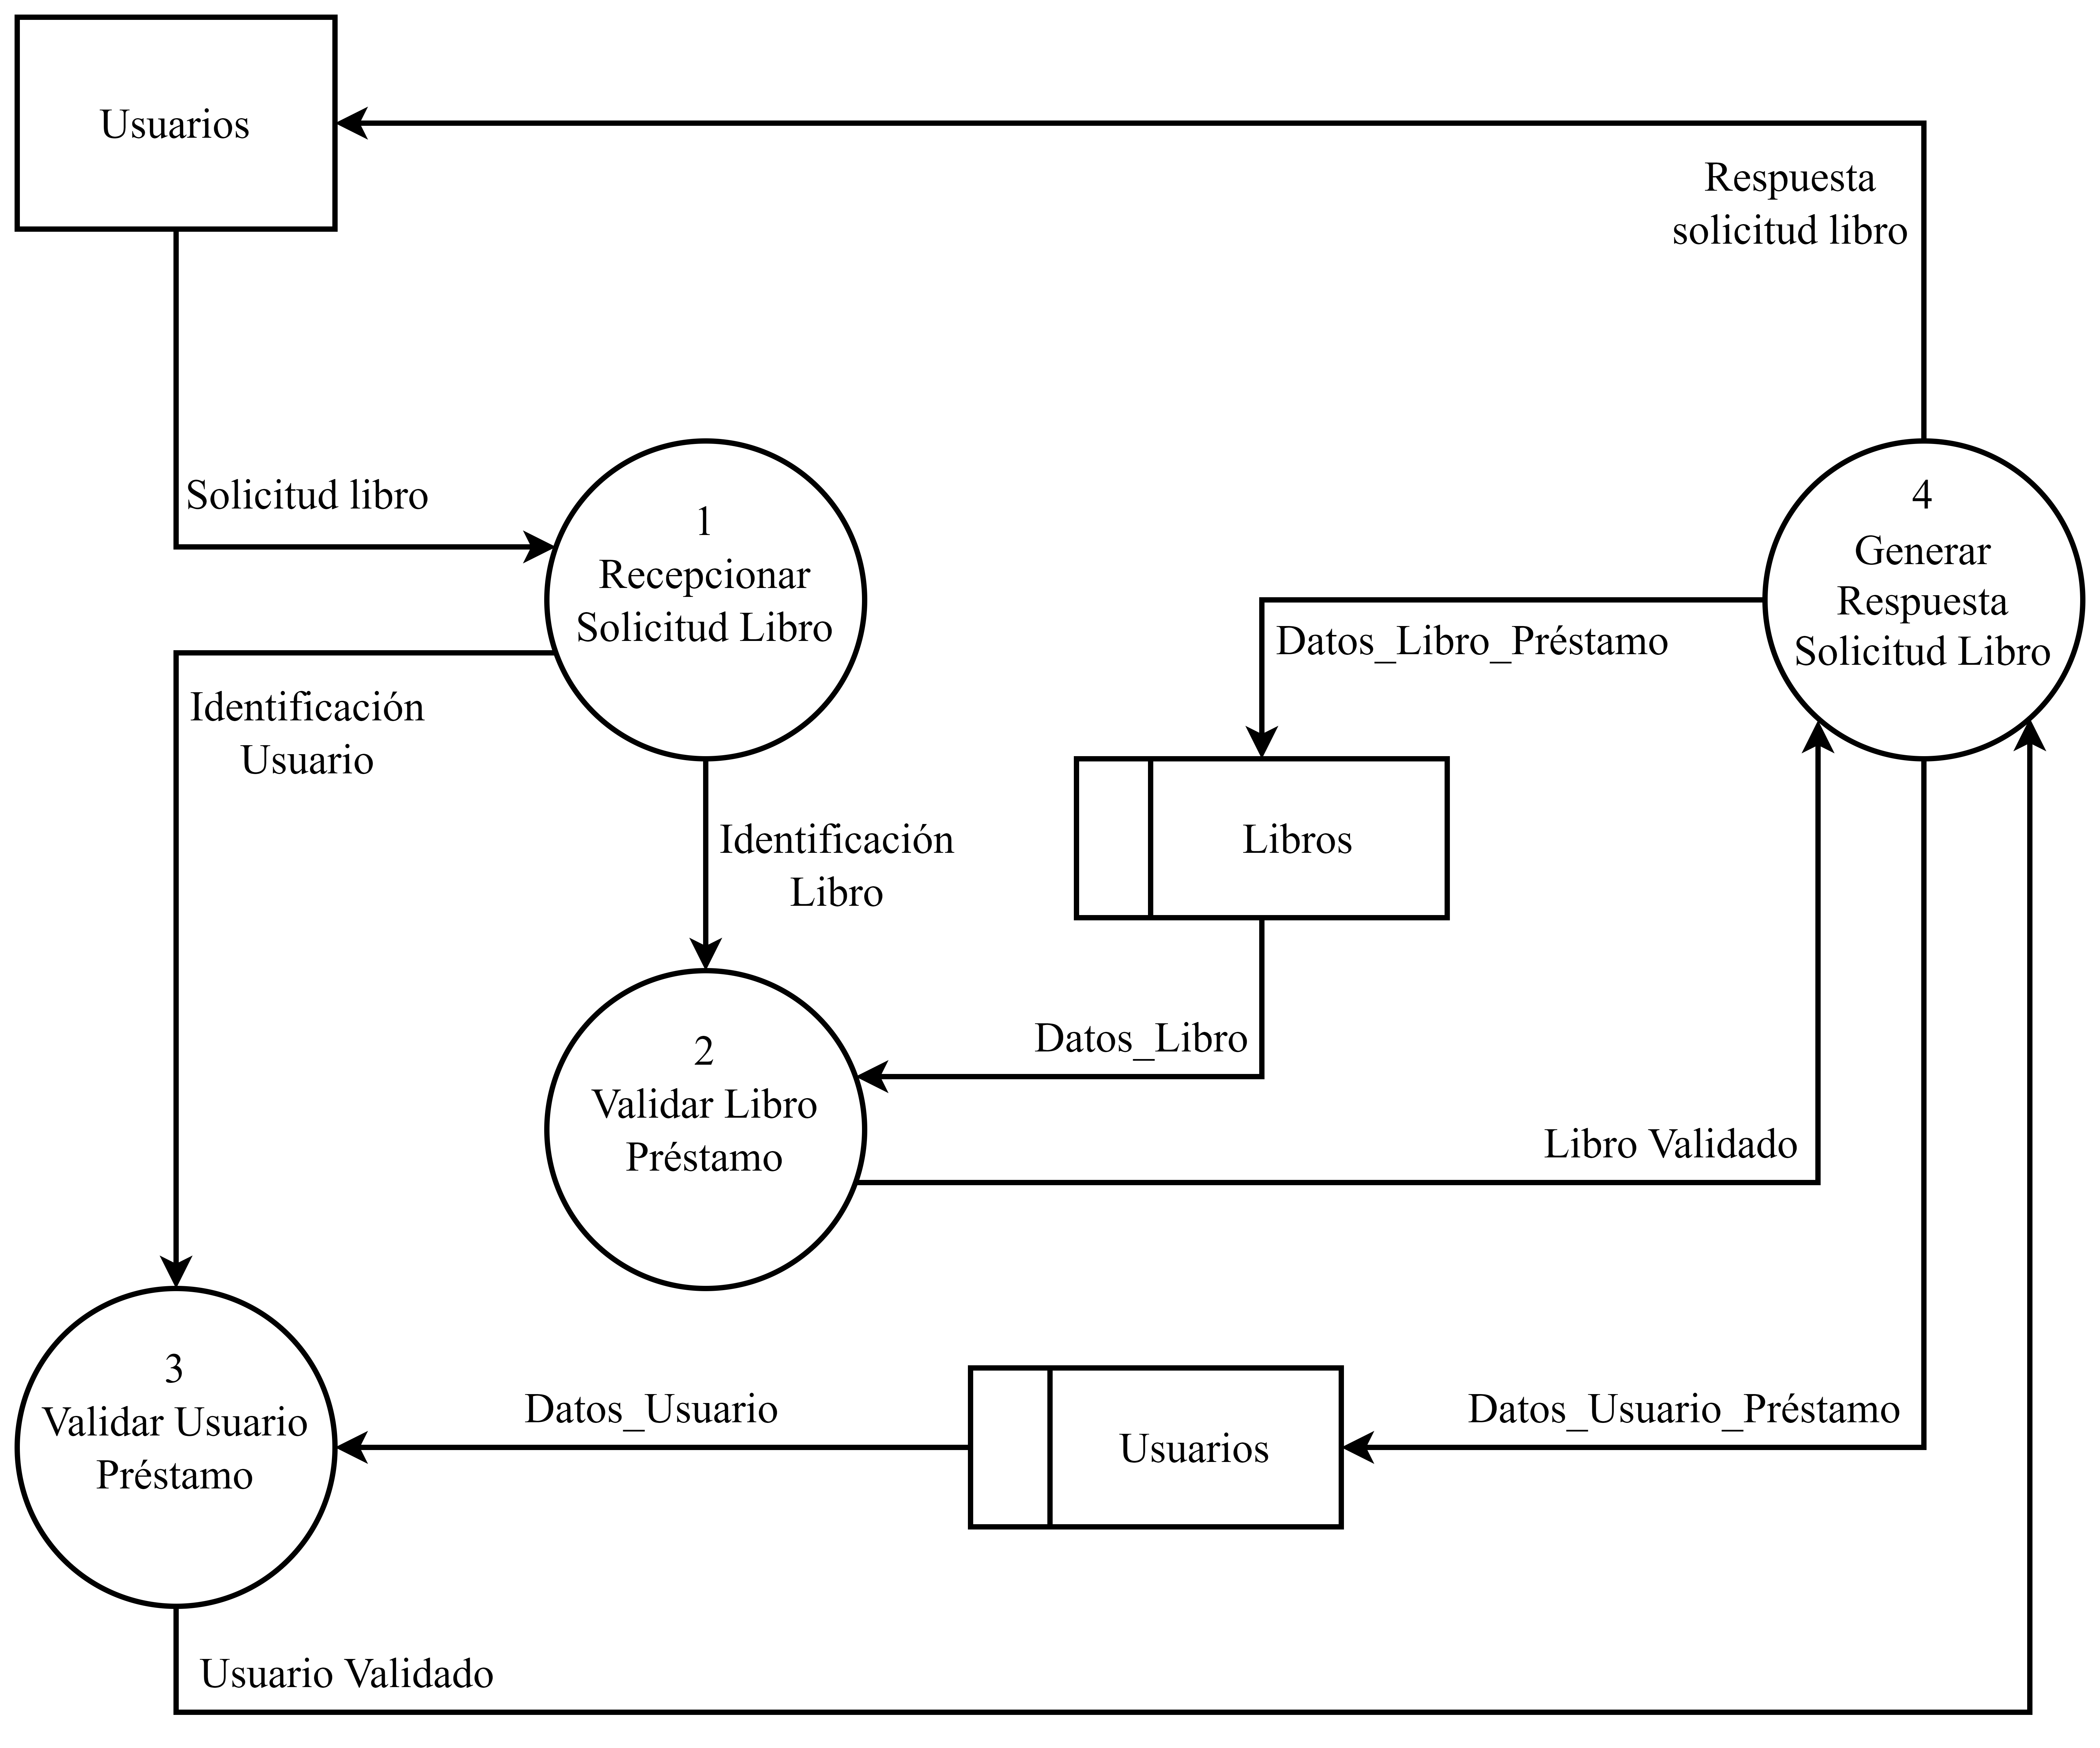
\includegraphics[width=\textwidth]{diagram/DFD2-Superior.png}
\end{figure}
\end{document}